\PassOptionsToPackage{dvipsnames}{xcolor}

\documentclass[10pt]{article} % For LaTeX2e
\usepackage[preprint]{tmlr}

% If accepted, instead use the following line for the camera-ready submission:
%\usepackage[accepted]{tmlr}
% To de-anonymize and remove mentions to TMLR (for example for posting to preprint servers), instead use the following:
%\usepackage[preprint]{tmlr}

\usepackage{amssymb,amsmath,amsthm,mathtools}
\usepackage{hyperref}
\usepackage{url}
\usepackage{upquote}
\usepackage{booktabs}

\usepackage{microtype}
\UseMicrotypeSet[protrusion]{basicmath} % disable protrusion for tt fonts

\usepackage{xcolor}

\usepackage{caption}
\usepackage{subcaption}

\usepackage{siunitx}

\usepackage{hyperref}
\hypersetup{
  colorlinks = true,
  breaklinks = true,
  linkcolor  = black,
  filecolor  = MidnightBlue,
  citecolor  = MidnightBlue,
  urlcolor   = MidnightBlue
}

\usepackage{cleveref}

\usepackage{todonotes}

% Optional math commands from https://github.com/goodfeli/dlbook_notation.
\input{math_commands.tex}
% operators
\DeclareMathOperator*{\argmax}{arg\,max}
\DeclareMathOperator*{\argmin}{arg\,min}
\DeclareMathOperator{\E}{E}
\DeclareMathOperator{\var}{Var}
\DeclareMathOperator{\cov}{Cov}
\DeclareMathOperator{\tr}{tr}
\DeclareMathOperator{\diag}{diag}
\DeclareMathOperator{\range}{range}
\DeclareMathOperator{\nullspace}{null}
\DeclareMathOperator{\rank}{rank}
\DeclareMathOperator{\card}{card}
\DeclareMathOperator{\sign}{sign}
\DeclareMathOperator{\st}{S}
\DeclareMathOperator{\normal}{Normal}
\DeclareMathOperator{\fnormal}{FoldedNormal}
\DeclareMathOperator{\bernoulli}{Bernoulli}
\DeclareMathOperator{\erf}{erf}
\DeclareMathOperator{\mse}{MSE}
\DeclareMathOperator{\risk}{R}
% \DeclareMathOperator{\I}{I}
% \DeclareMathOperator{\T}{}

\renewcommand{\vec}{\symbf}
\newcommand{\mat}{\symbf}
\newcommand*\du{\mathop{}\!\mathrm{d}}
\newcommand{\T}{\intercal}
\newcommand{\ones}{\symbf{1}}
\newcommand{\ind}[1]{\operatorname{I}_{#1}}

% \newcommand{\todojl}[1]{\todo[color=green!40]{#1}}

% \newcommand{\mv}[1]{{\boldsymbol{\mathrm{#1}}}}




\title{The Lasso and Ridge Regression Yield Biased Estimates of Imbalanced Binary Features}

% Authors must not appear in the submitted version. They should be hidden
% as long as the tmlr package is used without the [accepted] or [preprint] options.
% Non-anonymous submissions will be rejected without review.

\author{%
  \name Johan Larsson \email johan.larsson@stat.lu.se\\
  \addr Deparment of Statistics\\Lund University
  \AND
  \name Jonas Wallin \email jonas.wallin@stat.lu.se\\
  \addr Department of Statistics\\Lund University
}

\newcommand{\fix}{\marginpar{FIX}}
\newcommand{\new}{\marginpar{NEW}}

\def\month{MM}  % Insert correct month for camera-ready version
\def\year{YYYY} % Insert correct year for camera-ready version
\def\openreview{\url{https://openreview.net/forum?id=XXXX}} % Insert correct link to OpenReview for camera-ready version

\begin{document}

\maketitle

\begin{abstract}
  Regularized models are often sensitive to the scales of the features in the data. It has
therefore become standard practice to normalize (center and scale) features before fitting
the model. There are, however, many different ways to normalize the features and the choice
you make may have dramatic effects on the resulting model. For the lasso, for instance,
entirely different sets of features may be selected depending on which type of
normalization is used. In spite of this, the interplay between normalization and
regularization has not been studied previously. In this paper, we begin to bridge this
knowledge gap by studying binary and normally distributed features in the context of lasso,
ridge, and elastic net regression. We show that the class balances of binary features
directly influences the corresponding regression coefficients and this effect depends on
the combination of normalization strategy and regularization method (lasso, ridge, or
elastic net) used. We moreover show that this bias can be mitigated by scaling binary
features with their variance in the case of the lasso and standard deviation in the case of
ridge regression, but that this comes at the cost of increased variance. For the elastic
net, we demonstrate that scaling the penalty weights, rather than the features, can achieve
the same effect. We also tackle the case of mixes of binary and normal features as well as
interactions and provide some intial results on how to normalize features in these cases.

\end{abstract}

\section{Introduction}

When the data you want to model is high-dimensional, that is, the number of features \(p\) exceed the number of observations \(n\), it is impossible to apply classical statistical models such as standard linear regression since the design matrix \(\mat X\) is no longer of full rank. A common remedy to this problem is to \emph{regularize} the model by adding a term to the objective function that punishes models with large coefficients (\(\vec\beta\)). If we let \(h(\vec\beta; \mat X, \vec y)\) be the original objective function---which when minimized improves the model's fit to the data (\(\mat X, \vec y\))---then
\[
  f(\beta_0, \vec\beta; \mat X, \vec y) = h(\beta_0, \vec\beta; \mat X, \vec y) + g(\vec\beta)
\]
is a composite function within which we have added a penalty term \(g(\vec\beta)\).
In contrast to \(h\), this penalty depends only on the coefficients (\(\vec{\beta}s\)).
The intercept, \(\beta_0\), is not typically penalized.

Some of the most common penalties are the \(\ell_1\) and \(\ell_2\) penalties, that is \(g(\vec\beta) = \lVert \vec\beta \rVert_1\) or \(g(\vec\beta) = \lVert \vec\beta \rVert_2^2/2\)\footnote{Division by two in this case is used only for convenience.}, which, if \(h\) is the standard ordinary least-squares objective, represent lasso~\citep{tibshirani1996,santosa1986,donoho1994} and ridge (Tikhonov) regression respectively.
Other common penalities include SLOPE~\citep{bogdan2013,bogdan2015}, MCP~\citep{zhang2010}, hinge loss (used in support vector machines~\citep{cortes1995}) and SCAD~\citep{fan2001}.
Many of these penalities---indeed all of the previously mentioned ones---shrink coefficients in proportion to their sizes.

% TODO: Maybe say something about ℓ₀ (best subset) regularization

The issue with this type of shrinkage is that it is typically sensitive to the scales and locations of the features in \(\mat X\).
A common remedy is to \emph{normalize} the features before fitting the model by translating and dividing each column by respective translation and scaling factors.
For some problems, such factors may arise naturally from knowledge of the problem at hand.
A researcher may for instance have collected data on coordinates within a limited area and know that the coordinates are measured in meters.
Often, however, these scaling and location factors must be estimated from data.
The most popular choices for this type of scaling are based only on the marginal distributions of the features.
Some types of normalization, such as that applied in the adaptive lasso\footnote{The adaptive lasso typically uses estimates of the regression coefficients, typically from ordinary-least squares or ridge regression, to scale the features with.}~\citep{zou2006}, however, are based on the conditional distributions of the features and the response.
After fitting the model, the estimated coefficients are then usually returned to their original scale.

Another reason for normalizing the features is to improve the performance and stability of optimization algorithms used to fit the model.
We will not cover this aspect in this paper, but note that it is an important one.

In most sources and discussions on regularized methods, normalization is typically treated as a preprocessing step---separate from modeling. As we will show in this paper, however, the type of normalization used can have a critical effect on the estimated model, sometimes leading to entirely different conclusions with regard to feature importance as well as predictive performance. As a first example of this, consider \Cref{fig:realdata-paths}, which displays the lasso paths for three real data sets and three different types of normalization. Each panel shows the union of the first five predictors picked by either type of normalization. As we can see, the choice of normalization can have a significant impact on the estimated model. In the case of the \texttt{leukemia} data set, for instance, the models are starkly different with respect to both the identities of the features selected as well as their signs and magnitudes.

\begin{figure}[bpt]
  \centering
  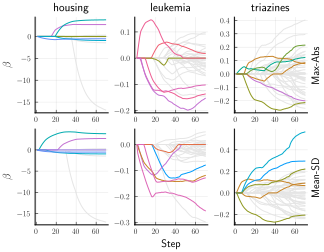
\includegraphics[]{plots/realdata_paths.pdf}
  \caption{%
    A display over the first predictors selected by the lasso for each type of normalization. Each panel shows the union of the first five predictors picked by either type of normalization.
  }
  \label{fig:realdata-paths}
\end{figure}

In addition, discussions on the choice of normalization are often focused on computational aspects and data storage requirements, rather than on the statistical properties of the choice of normalization. In our paper, we will argue that normalization should rather we considered as an integral part of the model. And that it for instance is unreasonable to base the choice of normalization on the type of data storage, which implicitly encodes the belief that a data set stored as a sparse matrix is somehow fundamentally different from a data set stored as a dense matrix.

\section{Preliminaries}

Throughout this paper, we assume that the data is generated from a linear model, \(y_i =
\beta_0^* + \vec x_i^\T \vec\beta^* + \varepsilon_i\) for \(i \in [n]\) where \([n] =
\{1,2,\dots,n\}\) and we use \(\beta_0^*\) and \(\vec\beta^*\) to denote the true intercept
and coefficients, respectively, and \(\varepsilon_i\) to denote measurement noise. \(\mat
X\) is the \(n \times p\) design matrix with features \(\vec x_j\) and \(\vec y\) the \(n
\times 1\) response vector. Furthermore, we use \(\hat\beta_0\) and \(\hat{\vec{\beta}}\)
to denote our estimates of the intercept and coefficients. Unless we state otherwise, we
assume \(\mat{X}\), \(\beta_0^*\), and \(\vec{\beta}^*\) to be fixed.%

There is much ambiguity regarding key terms in the field of normalization. \emph{Scaling},
\emph{standardization}, and \emph{normalization} are for instance used interchangeably
throughout the literature. Here, we define \emph{normalization} as the process of centering
and scaling the feature matrix, which we now formalize.

\begin{definition}[Normalization]
  \label{def:normalization}
  % Let \(\mat S\) be the \emph{scaling matrix}, which is a \(p \times p\) diagonal matrix with entries \(s_1, s_2, \dots, s_p\). Let \(\mat C\) be the \emph{centering matrix}, which is an \(n \times p\) matrix with each row equal to \([c_1, c_2, c_n]^\T\). Then the \emph{normalized design matrix} \(\tilde{\mat X}\) is defined as \(\tilde{\mat X} = (\mat X - \mat C)\mat S^{-1}\).
  Let \(\tilde{\mat X}\) be the normalized feature matrix, with elements \(\tilde{x}_{ij} =
  (x_{ij} - c_{j})/s_j,\) where \(x_{ij}\) is an element of the (unnormalized) feature matrix
  \(\mat{X}\) and \(c_j\) and \(s_j\) are the \emph{centering} and \emph{scaling} factors
  respectively.
\end{definition}

Some authors refer to the procedure in \Cref{def:normalization} as \emph{standardization},
but here we define standardization only as the case when centering with the mean and
scaling with the (uncorrected) standard deviation.

\subsection{Types of Normalization}

There are many different strategies for normalizing the design matrix. We list a few common
choices in \Cref{tab:normalization-types}. Standardization is perhaps the most popular type
of normalization, at least in the field of statistics. One of its benefits is that it
simplifies certain aspects of fitting the model, such as fitting the intercept. The
downside of standardization is that it involves centering by the mean, which destroys
sparsity. This is not a problem when \(\bm{X}\) is stored as a dense matrix; but when the
data is sparse, it may increase memory use and processing time.

% TODO: move to appendix?
\begin{table}[hbt]
  \centering
  \caption{
    Common ways to normalize a matrix of features using centering and scaling
    factors \(c_j\) and \(s_j\), respectively. Note that \(\bar{x}_j =
    n^{-1}\sum_{i=1}^n x_{ij}\).
  }
  \label{tab:normalization-types}
  \vskip 0.15in
  \small
  \begin{tabular}{lll}
    \toprule
    Normalization            & \(c_{j}\)          & \(s_j\)                                                   \\
    \midrule
    Standardization          & \(\bar{x}_j\)      & \(\sqrt{\frac{1}{n}\sum_{i=1}^n (x_{ij} - \bar{x}_j)^2}\) \\
    \addlinespace
    Max--Abs                 & 0                  & \(\max_i|x_{ij}|\)                                        \\
    \addlinespace
    Min--Max                 & \(\min_i(x_{ij})\) & \(\max_i(x_{ij}) - \min_i(x_{ij})\)                       \\
    \addlinespace
    \(\ell_1\)-Normalization & 0 or \(\bar{x}_j\) & \(\lVert \vec{x}_j\rVert_1\)                              \\
    \addlinespace
    Adaptive Lasso           & 0                  & \(\beta_j^\text{OLS}\)                                    \\
    \bottomrule
  \end{tabular}
\end{table}

When the data is sparse, a common alternative to standardization is to scale features by
their maximum absolute values (max--abs normalization). This method has no impact on binary
data\footnote{Except in the extreme case when all values are 0.} and therefore retains
sparsity. For other types of data, it scales the features to take values in the range
\([-1, 1]\). Since the scaling is determined by a single value for each feature, the method
is naturally sensitive to outliers. For many types of data, such as normally distributed
data, it is also often the case that the sample maximum depends on sample size, which often
makes use of the method problematic~(\Cref{thm:maxabs-gev}~(\Cref{sec:additional-theory})

% TODO: should we study l1-normalization more?
Min-max normalization scales the data to lie in \([0, 1]\). As with the max--abs method,
min-max normalization retains sparsity and also shares its sensitivity to outliers and
sample size. Unlike max--abs scaling, however, min--max scaling is not sensitive to the
\emph{location} of the data, only its \emph{spread}. In \(\ell_1\)-normalization, each
feature is scaled with its sum of absolute value. The method is common in signal
processing. A special case of normalization is the adaptive lasso~\citep{zou2006}, which is
a two-step procedure. First we fit a model such as ordinary least-squares (OLS) or ridge
regression. Then we use the estimated coefficients to scale the features and refit.

\subsection{The Lasso, Ridge Regression, and the Elastic Net}

Let \((\hat{\beta}_0^{(n)}, \hat{\vec{\beta}}^{(n)})\) be a solution to the problem in
\Cref{eq:elastic-net}. Expanding \(f\) in \Cref{eq:elastic-net}, we have
\[
  \begin{aligned}
     & \frac{1}{2}\left( \vec y^\T \vec y - 2(\tilde{\mat{X}}\vec{\beta} + \beta_0)^\T\vec{y} + (\tilde{\mat{X}}\vec{\beta} + \beta_0)^\T(\tilde{\mat{X}}\vec{\beta} + \beta_0)\right) \\
     & + \lambda_1 \lVert \vec\beta \rVert_1 + \frac{\lambda_2}{2}\lVert \vec \beta \rVert_2^2.
  \end{aligned}
\]
Taking the subdifferential with respect to \(\vec{\beta}\) and \(\beta_0\), the KKT
stationarity condition yields the following system of equations:
\begin{equation}
  \label{eq:kkt-elasticnet}
  \begin{cases}
    \tilde{\mat{X}}^\T(\tilde{\mat{X}}\vec{\beta} + \beta_0 - \vec{y}) + \lambda_1 g + \lambda_2 \vec\beta \ni \vec{0}, \\
    n \beta_0 + (\tilde{\mat{X}}\vec{\beta})^\T \vec{1} - \vec{y}^\T \vec{1} = 0,
  \end{cases}
\end{equation}
where \(g\) is a subgradient of the \(\ell_1\) norm that has elements \(g_i\) such that
\[
  g_i \in
  \begin{cases}
    \{\sign{\beta_i}\} & \text{if } \beta_i \neq 0, \\
    [-1, 1]            & \text{otherwise}.
  \end{cases}
\]

\subsection{Weighted Penalization}%
\label{sec:weighted-elasticnet}

One alternative to normalization, which will be of particular interest in the case of the
elastic net, is to weight the coefficients in the penalty term---and instead of minimizing
\Cref{eq:elastic-net} minimize the following objective:
\[
  \begin{multlined}
    \tilde{f}(\beta_0, \vec{\beta}, \mat{X}, \vec{y}, \lambda_1, \lambda_2) =\\
    \frac{1}{2} \lVert \vec{y} - \beta_0 - \mat{X}\vec{\beta}\rVert_2^2 + \lambda_1 \sum_{j=1}^p u_j |\beta_j| + \frac{\lambda_2}{2} \sum_{j=1}^p v_j \beta_j^2,
  \end{multlined}
\]
with \(\vec{u}\) and \(\vec{v}\) being \(p\)-length vectors of positive scaling factors. We
call this the \emph{weighted elastic net}, which is equivalent to the original form when
\(u_j = s_j\) and \(v_j = s_j^2\), which can be seen by substituting \(\beta_js_j =
\tilde{\beta}_j\) in \Cref{eq:elastic-net} and solving for \(\tilde{\vec{\beta}}\).

\subsection{Orthogonal Features}

If the features of the normalized design matrix are orthogonal, that is,
\(\tilde{\mat{X}}^\intercal \tilde{\mat{X}} = \diag\left(\tilde{\vec{x}}_1^\T
\tilde{\vec{x}}_1, \dots, \tilde{\vec{x}}_p^\intercal \tilde{\vec{x}}_p\right) \), then
\Cref{eq:kkt-elasticnet} can be decomposed into a set of \(p + 1\) conditions:
%
\[
  \begin{cases}
    \tilde{\vec{x}}_j^\T (\tilde{\vec{x}}_j \beta_j + \ones \beta_0 - \vec{y}) + \lambda_2 \beta_j + \lambda_1 g \ni 0, & j \in [p], \\
    n \beta_0 + (\tilde{\mat{X}}\vec{\beta})^\T \vec{1} -  \vec{y}^\T \ones = 0.
  \end{cases}
\]
%
The inclusion of the intercept ensures that the locations (means) of the features do not
affect the solution (except for the intercept itself). We will therefore from now on assume
that the features are mean-centered so that \(c_j = \bar{\vec{x}}_j\) for all \(j\) and
therefore \(\tilde{\vec{x}}_j^\T \ones = 0\). A solution to the system of equations is then
given by the following set of equations~\citep{donoho1994}:
%
\begin{equation*}
  \label{eq:orthogonal-solution-normalized}
  \hat{\beta}^{(n)}_j = \frac{\st_{\lambda_1}\left(\tilde{\vec{x}}_j^\T \vec{y}\right)}{\tilde{\vec{x}}_j^\T \tilde{\vec{x}}_j + \lambda_2},
  \qquad
  \hat{\beta}_0^{(n)} = \frac{\vec{y}^\T \ones}{n},
\end{equation*}
%
where \(\st_\lambda(z) = \sign(z) \max(|z| - \lambda, 0)\) is the soft-thresholding
operator.

\subsection{Rescaling Regression Coefficients}

Normalization changes the optimization problem and its solution, the coefficients, which
will now be on the scale of the normalized features. But we are interested in
\(\hat{\vec{\beta}}\): the coefficients on the scale of the original problem. To obtain
these, we transform the coefficients from the normalized poblem, \(\hat\beta^{(n)}_j\),
back via
%
\begin{equation}
  \label{eq:orthogonal-solution}
  \hat\beta_j = \frac{\hat\beta^{(n)}_j}{s_j} \quad\text{for}\quad j = 1,2,\dots,p.
\end{equation}
%
There is a similar transformation for the intercept but we omit here since we are not
interested in it. Note that this rescaling is not needed in the weighted elastic
net~(\Cref{sec:weighted-elasticnet}), since the estimated coefficients are kept on the same
scale as the original (non-normalized) data.

\section{Bias and Variance of the Elastic Net Estimator}%
\label{sec:theory}

Now, assume that \(\mat{X}\) is fixed and that \(\vec{y} = \mat{X}\vec{\beta} +
\vec{\varepsilon}\), where \(\varepsilon_i\) is identically and independently distributed
noise with mean zero and finite variance \(\sigma_\varepsilon^2\). As in
\Cref{sec:elastic-net-solution}, we will also assume that the features are orthogonal,
which means that the solution is given directly by
\Cref{eq:orthogonal-solution-normalized}:
\[
  \hat{\beta}_j = \frac{\st_{\lambda_1}({Z_j})}{d_j}\quad\text{with}\quad d_j = s_j(\tilde{\vec{x}}_j^\T \tilde{\vec{x}}_j + \lambda_2).
\]
We can then show that
\begin{equation}
  \label{eq:z-d}
  \tilde{\vec{x}}_j^\T \vec{y} = \frac{\beta_j^* n \nu_j- \vec{x}_j^\T \vec{\varepsilon}}{s_j}
  \quad\text{and}\quad
  d_j = s_j\left(\frac{n \nu_j}{s_j^2} + \lambda_2\right),
\end{equation}
where \(\nu_j\) is the uncorrected sample variance of \(\vec{x}_j\).
The bias and variance of \(\hat{\beta}_j\) are given by
\begin{align*}
  % \bias(\hat{\beta}_j; \beta_j^*) & = \frac{1}{d_j}\E \st_\lambda(\tilde{\vec{x}}_j^\T \vec{y}) - \beta^*_j, \\
  \E \hat\beta_j - \beta_j^* & = \frac{1}{d_j}\E \st_\lambda(\tilde{\vec{x}}_j^\T \vec{y}) - \beta^*_j, \\
  \var \hat\beta_j           & = \frac{1}{d_j^2} \var \st_\lambda(\tilde{\vec{x}}_j^\T \vec{y}).
\end{align*}
See \Cref{sec:bias-var-deriv} for a derivation of the results above
as well as expressions for \(\E \st_\lambda(x)\) and \(\var S_\lambda(x)\).

Note that these expressions hold for a general distribution on the error term. From now on,
however, we will assume that \(\vec{\varepsilon}\) is normally distributed, under which the
bias and variance of \(\hat{\beta}_j\) has an analytical
expression~(\Cref{sec:normally-distributed-noise}).

\subsection{Binary Features}%
\label{sec:theory-binary-features}

The main focus in this paper is the case when \(\bm{x}_j\) is a binary feature, such that
\(x_{ij} \in \{0, 1\}\) for all \(i\). We define the \emph{class balance} of this feature
as \(q_j = \bar{\bm{x}}_j\): the proportion of ones. For the majority of our results it
would make no difference if we were to swap the ones and zeros as long as an intercept is
included, and ``class balance'' is then equivalent to the proportion of either. But later
on, as we turn to the case of interactions in \Cref{sec:interactions}, we will see that the
choice then matters.

In the case of binary features, inserting \(\nu_j = (q_j - q_j^2)\) (the uncorrected sample
variance for a binary feature) into \Cref{eq:z-d} yields
\begin{align*}
  \tilde{\vec{x}}_j^\T \vec{y} & = \frac{\beta_j^* n(q_j - q_j^2) - \vec{x}_j^\T \vec{\varepsilon}}{s_j}, \\
  d_j                          & = s_j \left(\frac{n(q_j - q_j^2)}{s_j^2} + \lambda_2\right),
\end{align*}
% \[
%   \begin{aligned}
%     \tilde{\vec{x}}_j^\T \tilde{\vec{x}}_j & = \frac{1}{s_j^2}(\vec{x}_j - \ones c_j)^\T (\vec{x}_j - \ones c_j) = \frac{1}{s^2_j}(nq - 2nq_j^2 + nq_j^2) = \frac{nq_j(1-q_j)}{s^2_j}, \\
%     \tilde{\vec{x}}_j^\T \vec{x}_j         & = \frac{1}{s_j}(\vec{x}_j^\T \vec{x}_j - \vec{x}_j^\T \ones c_j) = \frac{nq_j(1 - q_j)}{s_j}.
%   \end{aligned}
% \]
and consequently
\[
  \mu_j = \frac{\beta^*_j n(q_j - q_j^2)}{s_j}\quad \text{and} \quad \sigma_j^2 = \frac{\sigma_\varepsilon^2n(q_j- q_j^2)}{s^2_j}.
\]
%
We obtain the expected value of the elastic net estimate with respect to \(q_j\) by
inserting \(\mu_j\) and \(\sigma_j\) into \Cref{eq:mean-centered-eval}.

The presence of the factor \(q_j - q_j^2\) in \(\mu_j\), \(\sigma_j^2\), and \(d_j\)
indicates a link between class balance and the elastic net estimator and that this
relationship is mediated by the scaling factor \(s_j\). To achieve some initial intuition
for this relationship, we consider the noiseless case (\(\sigma_\varepsilon = 0\)) in
which, we have
\begin{equation}
  \label{eq:noiseless-estimator}
  \hat{\beta}_j = \frac{\st_{\lambda_1}(\tilde{\vec{x}}_j^\intercal \vec{y})}{s_j\left(\tilde{\vec{x}}_j^\intercal \tilde{\vec{x}}_j + \lambda_2\right)}
  =
  \frac{\st_{\lambda_1}\left(\frac{\beta_j^* n (q_j - q_j^2)}{s_j}\right)}{s_j\left(\frac{n(q_j - q_j^2)}{s_j^2} + \lambda_2\right)}.
\end{equation}
%
This expression shows that class balance directly affects the estimator. For values of
\(q_j\) close to \(0\) or \(1\), the input into the soft-thresholding part of the estimator
diminishes and consequently forces the estimate to zero, that is, unless we use the scaling
factor \(s_j = q_j - q_j^2\), in which case the soft-thresholding part will be unaffected
by class imbalance. This choice will not, however, mitigate the impact of class imbalance
on the ridge part of the estimator, for which we would instead need \(s_j = (q_j -
q_j^2)^{1/2}\). For any other choices, \(q_j\) will affect the estimator through both the
ridge and lasso parts, which means that there exists no scaling \(s_j\) that will mitigate
the bias in this case. Later on in \Cref{sec:binary-weighting} we will show how to tackle
this issue for the elastic net by scaling the penalty term individually for each feature.
For now, however, we will continue with the case of normalization.

Based on this reasoning, we will consider the scaling parameterization \(s_j =
(q_j-q_j^2)^\delta\), \(\delta \geq 0\). This includes the cases that we are primarily
interested in, namely \(\delta = 0\) (no scaling), \(\delta = 1/2\) (standard-deviation
scaling), and \(\delta = 1\) (variance scaling). Note that the last of these types,
variance scaling, is not a standard type of normalization; yet, as we have already seen, it
has some interesting properties in the context of binary features.

Another interesting fact about \Cref{eq:noiseless-estimator}, which holds also in the noisy
situation, is that even when the binary feature is balanced (\(q_j = 1/2\)), normalization
will still have an effect on the estimator. Using \(\delta = 0\), for instance, leads the
true coefficient \(\beta_j^*\) in the input to \(\st_\lambda\) to be scaled by \(n (q_j -
q_j^2) = n/4\). For \(\delta = 1\) there would in contrast be no scaling in the
class-balanced case. And for \(\delta = 1/2\), the scaling factor is \(n/2\). Generalizing
this we see that to achieve equivalent scaling in the class-balanced case for all types of
normalization, under our parameterization, we would need to use \(s_j = 4^{\delta - 1} (q_j
- q_j^2)^\delta\). But this only resolves the issue for the lasso. To achieve a similar
effect for ridge regression, we would need another (but similar) modification. Since all
features are binary under our current assumptions we will for now just scale \(\lambda_1\)
and \(\lambda_2\) to account for this effect,\footnote{We use this strategy in all of the
  following examples.} which is equivalent to modifying \(s_j\). We will return to this issue
in \Cref{sec:mixed-data}, when we consider mixes of binary and normal features, in which
case this has significant implications.

We now leave the noiseless scenario and proceed to consider how class balance affects the
bias, variance, and selection probability of the elastic net estimator, starting with the
latter. A consequence of the normal error distribution and consequent normal distribution
of \({Z_j}\) is that the probability of selection in the elastic net problem is given by
\begin{align}
  \label{eq:selection-probability}
   & \Pr\left(\hat{\beta}_j \neq 0\right) =                                                                                                       \nonumber
  \\
  % & = \Pr\left(\st_{\lambda_1}({Z_j}) \neq 0\right)                                                                                                                                                                                                                           \nonumber \\
  %                                      & = \Pr\left({Z_j} > \lambda_1\right) + \Pr\left({Z_j} < -\lambda_1\right)                                                                                                                                                                                                  \nonumber \\
  %                                      & = \cdf\left(\frac{\mu_j - \lambda_1}{\sigma_j}\right) + \cdf\left(\frac{- \mu_j -\lambda_1}{\sigma_j}\right)                                                                                                                                                              \nonumber \\
   & \cdf \left( \frac{\beta_j^*n (q_j-q_j^2)^{1/2} - \lambda_1(q_j-q_j^2)^{\delta - 1/2}}{\sigma_\varepsilon \sqrt{n}}\right)                \nonumber     \\
   & + \cdf \left( \frac{-\beta_j^*n (q_j-q_j^2)^{1/2} - \lambda_1(q_j-q_j^2)^{\delta - 1/2}}{\sigma_\varepsilon \sqrt{n}}\right).
\end{align}
Letting \(\theta_j = -\mu_j - \lambda_1 \) and \(\gamma_j = \mu_j - \lambda_1\), we can
express this probability asymptotically as \(q_j \rightarrow 1^+\) as
\begin{equation}
  \label{eq:selection-probability-limit}
  \lim_{q_j \rightarrow 1^+} \Pr(\hat{\beta}_j \neq 0) =
  \begin{cases}
    0                                                                & \text{if } 0 \leq \delta < \frac{1}{2}, \\
    2\cdf\left(-\frac{\lambda_1}{\sigma_\varepsilon \sqrt{n}}\right) & \text{if } \delta = \frac{1}{2},        \\
    1                                                                & \text{if } \delta > \frac{1}{2}.
  \end{cases}
\end{equation}

In \Cref{fig:selection-probability}, we plot this probability for various settings of
\(\delta\) for a single feature. Our intuition from the noiseless case holds: suitable
choices of \(\delta\) can mitigate the influence of class imbalance on selection
probability. The lower the value of \(\delta\), the larger the effect of class imbalance
becomes. Note that the probability of selection initially decreases also in the case when
\(\delta \geq 1\). This is a consequence of increased variance of \({Z_j}\) due to the
scaling factor that scales the measurement noise \(\sigma_\varepsilon^2\) upwards. Then, as
\(q_j\) approaches 1, the probability picks up again and eventually approaches 1 for
\(\delta \in \{1, 1.5\}\). The reason for this is that the variance of \({Z_j}\) eventually
explodes (again due to the scaling), which ultimately removes the soft-thresholding effect
altogether. Note that the selection probability is unaffected by \(\lambda_2\).

\begin{figure}[htpb]
  \centering
  \includegraphics[]{plots/selection_probability.pdf}
  \caption{%
    Probability of selection in the lasso given measurement noise
    % TODO: what is \lambda1 set to here?
    \(\sigma_\varepsilon\), regularization level \(\lambda_1\), and class
    balance \(q\). The scaling factor is set to \(s_j = (q - q^2)^\delta\),
    \(\delta \geq 0\). The dotted line represents the asymptotic limit for
    \(\delta = 1/2\)~(\Cref{eq:selection-probability-limit}).
    \label{fig:selection-probability}}
\end{figure}

Now we turn to the impact of class imbalance on bias and variance of the elastic net
estimator. We begin, in \Cref{thm:classbalance-bias}, by considering the expected value of
the elastic net estimator in the limit as \(q_j \rightarrow 1^+\).

\begin{theorem}
  \label{thm:classbalance-bias}
  If \(\vec{x}_j\) is a binary feature with class balance \(q_j \in (0, 1)\),
  \(\lambda_1 \in [0,\infty)\), \(\lambda_2 \in [0,\infty)\),
  \(\sigma_\varepsilon > 0\), and \(s_j = (q_j - q_j^2)^{\delta}\), \(\delta
  \geq 0\)  then
  \[
    \lim_{q_j \rightarrow 1^+} \E \hat{\beta}_j =
    \begin{cases}
      0                                                                                                  & \text{if } 0 \leq \delta < \frac{1}{2}, \\
      \frac{2n \beta_j^*}{n + \lambda_2} \cdf\left(-\frac{\lambda_1}{\sigma_\varepsilon \sqrt{n}}\right) & \text{if } \delta = \frac{1}{2},        \\
      \beta^*_j                                                                                          & \text{if } \delta > \frac{1}{2}.
    \end{cases}
  \]
\end{theorem}

\Cref{thm:classbalance-bias} shows that the bias of the elastic net estimator approaches
\(-\beta_j^*\) as \(q_j \rightarrow 1^+\) when \(0 \leq \delta < 1/2\). When \(\delta =
1/2\) (standardization), the estimate instead approaches the true coefficient scaled by the
probability that a standard normal variable is smaller than
\(\beta_j^*\sqrt{n}\sigma_\varepsilon^{-1}\). For \(\delta > 1/2\), the estimate is
asymptotically unbiased. This comes as a result of scaling the variance component from the
error term and is accompanied by exponentially increasing variance, which suggests that
variance-scaling may be problematic in the large noise--large imbalance scenario. In
\Cref{thm:classbalance-variance}, we continue by studying the variance in the limit as
\(q_j \rightarrow 1^+\).

\begin{theorem}
  \label{thm:classbalance-variance}
  Assume the conditions of \Cref{thm:classbalance-bias} hold, except that
  \(\lambda_1 > 0\). Then
  \[
    \lim_{q_j \rightarrow 1^+} \var \hat{\beta}_j =
    \begin{cases}
      0      & \text{if } 0 \leq \delta < \frac{1}{2}, \\
      \infty & \text{if } \delta \geq \frac{1}{2}.
    \end{cases}
  \]
\end{theorem}

Note that \Cref{thm:classbalance-variance} applies only to the case when \(\lambda_1 > 1\).
In \Cref{cor:ridge-variance}~(\Cref{sec:ridge-variance}), we state the corresponding result
for ridge regression.

\Cref{thm:classbalance-variance} formally proves the asymptotic variance effects of our
scaling parameter \(s_j\) which we have already discussed in the context of selection
probability and bias. Taken together with the results from \Cref{thm:classbalance-bias},
this suggests that the choice of scaling parameter, at least in the case of our specific
parameterization, introduces a bias--variance tradeoff with respect to \(\delta\): we can
reduce class imbalance-induced bias by increasing \(\delta\) but do so at the price of
increase variance.

In \Cref{fig:bias-var-onedim-lasso}, we now visualize bias, variance, and mean-squared
error for ranges of class balance and various noise-level settings for a lasso problem. The
figure demonstrates the bias--variance tradeoff that our asymptotic results suggest and
indicates that the optimal choice of \(\delta\) is related to the noise level in the data.
Since this level is unknown for most data and can only be estimated in the low-dimensional
setting, it suggests there might be value in selecting \(\delta\) through
hyper-optimization, which we consider in \Cref{sec:experiments-hyperparameter}.\footnote{In
  \Cref{sec:experiments-hyperparameter}, we experiment with this type of hyper-optimization.}
In \Cref{fig:bias-var-onedim-ridge-full} (\Cref{sec:additional-results-biasvar}) we show
results for ridge regression as well. As expected, it is then \(\delta = 1/2\) that leads
to unbiased estimates in this case.

\begin{figure}[htpb]
  \centering
  \includegraphics[]{plots/binary_onedim_bias_var_lasso_small.pdf}
  \caption{%
    Bias, variance, and mean-squared error for a one-dimensional lasso problem,
    parameterized by noise level (\(\sigma_\varepsilon\)), class balance (\(q\)), and
    scaling (\(\delta\)). Dotted lines represent asymptotic bias of the lasso
    estimator in the case when \(\delta = 1/2\). See \Cref{fig:bias-var-onedim-lasso-full}
    for extended results.}
  \label{fig:bias-var-onedim-lasso}
\end{figure}

So far, we have only considered a single binary feature. But under the assumption of
orthogonal features, it is straightforward to introduce multiple binary features. In
\Cref{sec:power-fdr-multiple}, we present results on power, false discovery rates, and
error in this scenario. Later in \Cref{sec:experiments} we will study binary features in
simulated experiments. For now, however, we turn to the case of mixed data.

\subsection{Mixed Data}%
\label{sec:mixed-data}

In this section we consider the case where features are made up of a mix of normal and
binary features. A fundamental problem is then deciding how to put binary and normal
features on the same scale in order to regularize each type of feature fairly. In principle
we need to match a one-unit change in the binary feature with some amount of change in the
normal feature. To setup this situation formally, we will say that the effects of a binary
feature \(\vec{x}_1\) and a normal feature \(\vec{x}_2\) are \emph{comparable} if
\(\beta^*_1 = \kappa \sigma \beta^*_2\), where \(\kappa > 0\) represents the number of
standard deviations of the normal feature we consider to be comparable to one unit on the
binary feature. We illustrate this notion of comparability by the following examples.

% TODO: illustrate this with a figure
\begin{example}
  Assume \(\kappa = 2\). If \(\vec{x}_2\) is sampled from
  \(\normal\left(\mu_j, \sigma^2 = (1/2)^2\right)\), then the effects of \(\vec{x}_1\) and
  \(\vec{x}_2\) are comparable if \(\beta_1^* = 2\sigma \beta_2^* = \beta_2^*\).
\end{example}
% \begin{example}
%   Assume \(\kappa = 1\). If \(\vec{x}_2\) is sampled from \(\normal(\mu,
%   \sigma^2 = 2^2)\), then the effects of \(\vec{x}_1\) and \(\vec{x}_2\) are comparable if
%   \(\beta_1^* = \sigma\beta_2^* = 2\beta_2^*\).
% \end{example}

The definition above refers to the true coefficients, but for our regularized estimates we
want \(\hat{\beta}_1 = \kappa\sigma\hat{\beta}_2\) to hold. If we assume that we are in a
noiseless situation (\(\sigma_\varepsilon = 0\), are standardizing the normal feature and
that, and that, for simplicity, \(\bm{x}_1\) has mean zero, then we need the following
equality to hold:
%
\begin{align}
  \label{eq:comparable-effects}
  \hat{\beta}_1                                                                                                                          & = \kappa\sigma \hat{\beta}_2                                                                                                                         & \implies \nonumber \\
  \frac{\st_{\lambda_1}(\tilde{\vec{x}}_1^\intercal \vec{y})}{s_1\left(\tilde{\vec{x}}_1^\intercal \tilde{\vec{x}}_1 + \lambda_2\right)} & =\frac{\kappa\sigma \st_{\lambda_1}(\tilde{\vec{x}}_2^\intercal \vec{y})}{s_2\left(\tilde{\vec{x}}_2^\intercal \tilde{\vec{x}}_2 + \lambda_2\right)} & \implies \nonumber \\
  \frac{\st_{\lambda_1}\left(\frac{n\beta_1^* (q - q^2)}{s_1}\right)}{s_1\left(\frac{n(q - q^2)}{s_1^2} + \lambda_2\right)}              & =  \frac{\kappa \st_{\lambda_1}\left(\frac{n\beta_1^*}{\kappa} \right)}{n + \lambda_2}.                                                              &
\end{align}
%
For the lasso (\(\lambda_2 = 0\)) and ridge regression (\(\lambda_1=0\)), we see that the
equation holds for \(s_1 = \kappa (q - q^2)\) and \(s_1 = (q - q^2)^{1/2}\), respectively.
In other words, we achieve comparability in the lasso by scaling each binary feature with
its variance times \(\kappa\). And for ridge regression, we can achieve comparability by
scaling with standard deviation, irrespective of \(\kappa\). For any other choices of
\(s_1\), equality holds only at a single fixed level of class balance. Let this level be
\(q_0\). Then, to achieve equality for \(\lambda_2 = 0\), we need \(s_1 =\kappa (q_0 -
q_0^2)^{1 - \delta}(q - q^2)^\delta\). Similarly, for \(\lambda_1 = 0\), we need \(s_1 =
(q_0 - q_0^2)^{1 - 2\delta} (q - q^2)^\delta\). In the sequel, we will assume that \(q_0 =
1/2\), to have effects be equivalent for the class-balanced case.

Note that this means that the choice of normalization has an implicit effect on the
relative penalization of binary and normal features, even in the class-balanced case (\(q_1
= 1/2\)). If we for instance use \(\delta=0\) and fit the lasso, then
\Cref{eq:comparable-effects} for a binary feature with \(q_1=1/2\) becomes
\(4\st_{\lambda_1}\left(n\beta_1^*/4\right) = \kappa \st_{\lambda_1}(n\beta_1^*/\kappa ),\)
which implies \(\kappa = 4\). In other words, the choice of normalization equips our model
with a belief about how binary and normal features should be penalized relative to one
another.

For the rest of this paper, we will use \(\kappa = 2\) and say that the effects are
comparable if the effect of a flip in the binary feature equals the effect of a
two-standard deviation change in the normal feature. We motivate this choice by an argument
of \citet{gelman2008}, who suggests that the classical use of standardized regression
coefficients to compare effects in a regression model is a default that unduly emphasizes
effects of continuous features for many real data sets. We want to stress that the choice
of \(\kappa\) should if possible be based on contextual knowledge of the data and that our
results depend only superficially on this particular setting. We do, however, want to
emphasize that this choice should be made \emph{actively} and not be allowed to implicitly
depend on the type of normalization used.

Finally, note that we assumed a noiseless case above. In the presence of noise, the bias
induced by the combination of noise level and normalization choice will affect these
results (see \Cref{fig:bias-var-onedim-lasso}), which means that normally distributed and
binary features will not be comparable in this case.

\subsection{Interactions}\label{sec:interactions}

The elastic net can be extended to include interactions. There is previous literature on
this topic~\citep{bien2013,zemlianskaia2022,lim2015}, but it has not considered the
possible influence of normalization. Here, we will consider simple pairwise interactions
with no restriction on the presence of main effects. For our analysis, we let \(\vec{x}_1\)
and \(\vec{x}_2\) be two features of the data and \(\bm{x}_3\) their interaction. Our model
is \(\bm{y}=\beta_0 + \bm{X\beta} + \bm{\varepsilon}\) as before, with \(\beta_3\)
representing the effect of the interaction.

We consider two cases in which we assume that the features are orthogonal and that
\(\vec{x}_1\) is binary with class balance \(q_1\). In the first case, we let \(\bm{x}_2\)
be normal with mean \(\mu\) and variance \(\sigma^2\), and in the second case \(\bm{x}_2\)
be binary with class balance \(q_2\). To construct the interaction feature, we center the
main features and then multiply element-wise. The elements of the interaction feature are
then given by \(x_{3,i} = (x_{1,i} - \bar{\bm{x}}_1)(x_{2,i} - \bar{\bm{x}}_2)\). The main
motivation for centering is that it removes correlation between the main features and the
interaction, which would otherwise affect the estimates due to the regularization.

Centering normal features is also important because it ensures that their means do not
factor into the estimation of their effects, which is otherwise the case since the variance
of \(\bm{x}_3\) would then be \(q_1(\sigma^2 + \mu^2(1 - q_1))\) in the case when
\(\bm{x}_1\) is centered and \((q_1 - q_1^2)(\sigma^2 + \mu^2)\) otherwise. Centering
binary features is also important because the variance of the interaction term is otherwise
\(q_1\sigma^2\) (provided \(\bm{x}_2\) is centered), which would mean that the
encoding\footnote{Whether values are \{0,1\} or \{-1, 1\} for instance.} of values of the
binary feature would directly affect the interaction term.

If \(\bm{x}_2\) is normal and both features are centered before computing the interaction
term, the variance becomes \(\sigma^2 (q-q^2)\), which suggests using \(s_3 = \sigma (q -
q^2)^\delta\) along the lines of our previous reasoning. And if \(\bm{x}_2\) is binary,
instead, then similar reasoning suggests using \(s_3 = ((q_1-q_1^2)(q_2-q_2^2))^\delta\).
In \Cref{sec:experiments-interactions}, we will study the effects of these choices in
simulated experiments.

\subsection{The Weighted Elastic Net}\label{sec:binary-weighting}

We have so far shown that certain choices of normalization can mitigate the class-balance
bias imposed by the lasso and ridge regularization. But we have also
demonstrated~(\Cref{sec:theory-binary-features}) that there is no (simple) choice of
scaling that can achieve the same effect for the elastic net.
\Cref{eq:noiseless-estimator}, however, suggests a natural alternative to normalization,
which is to use the weighted elastic net, in which we minimize
\[
  \frac{1}{2} \lVert \vec{y} - \beta_0 - \mat{X}\vec{\beta}\rVert_2^2 + \lambda_1 \sum_{j=1}^p u_j |\beta_j| + \frac{\lambda_2}{2} \sum_{j=1}^p v_j \beta_j^2,
\]
with \(\vec{u}\) and \(\vec{v}\) being \(p\)-length vectors of positive scaling factors.
This is equivalent to the standard elastic net for a normalized feature matrix when \(u_j =
s_j\) and \(v_j = s_j^2\), which can be seen by substituting \(\beta_js_j =
\tilde{\beta}_j\) in \Cref{eq:elastic-net} and solving for \(\tilde{\vec{\beta}}\). Note
that we do not need to rescale the coefficients from this problem as we would for the
standard elastic net on normalized data.

We can then control class-balance bias by setting our weights according to \(u_j = v_j =
(q_j - q_j^2)^{\omega}\) and counteract it, at least in the noiseless case, with \(\omega =
1\). For the lasso and ridge regression, this is equivalent to using \(\delta = 1\) and
\(\delta = 1/2\) respectively.

Results analogous to those in \Cref{sec:theory-binary-features} can be attained with a few
small modifications for the weighted elastic net case. Starting with selection probability,
we can set \(s_j = 1\) and replace \(\lambda_1\) with \(\lambda_1 u_j =
\lambda_1(q_j-q_j^2)^\omega\) in \Cref{eq:selection-probability}, which shows that
\(\omega\) and \(\delta\) have interchangeable effects for selection probability. Note that
this extends to the limit in \Cref{eq:selection-probability-limit}.

As far as expected value and variance of the weighted elastic net estimator is concerned,
the quantities in \Cref{eq:mean-centered-eval} and \Cref{eq:mean-centered-variance} apply
directly in the case of the weighted elastic net given \(s_j = 1\) for all \(j\) and
replacing \(\lambda_1\) as in the previous paragraph and \(\lambda_2\) with \(\lambda_2
(q_j - q_j^2)^\omega\). On the other hand, the asymptotic results differ slightly as we
will show next, starting with the expected value.

\begin{theorem}
  \label{thm:weighted-elasticnet-bias}
  Let \(\vec{x}_j\) be a binary feature with class balance \(q_j \in (0, 1)\) and take
  \(\lambda_1 > 0\), \(\lambda_2 > 0\), and \(\sigma_\varepsilon > 0\). For the
  weighted elastic net with weights \(u_j = v_j = (q_j-q_j^2)^\omega\) and \(\omega \geq 0\), it holds that
  \[
    \lim_{q_j \rightarrow 1^+} \E \hat{\beta}_j =
    \begin{cases}
      0                              & \text{if } 0 \leq \omega < 1, \\
      \frac{\beta^*n}{n + \lambda_2} & \text{if } \omega = 1,        \\
      \beta^*                        & \text{if } \omega > 1,
    \end{cases}
  \]
  \[
    \lim_{q_j \rightarrow 1^+} \var \hat{\beta}_j =
    \begin{cases}
      0      & \text{if } 0 \leq \delta < \frac{1}{2}, \\
      \infty & \text{if } \delta \geq \frac{1}{2}.
    \end{cases}
  \]
\end{theorem}

This result is similar to the one for the unweighted but normalized elastic net. The only
difference arises in the case when \(\omega = 1\), in which case the limit is unaffected by
\(\lambda_1\) in the case of the weighted elastic net.

This result mimics the result for asymptotic variance in the case of the unweighted elastic
net with normalization. In \Cref{fig:binary-onedim-bias-var-elnet}, we plot bias, variance,
and mean-squared error for the weighted elastic net. Again, we see that the behavior of
bias as \(q_j \rightarrow 1^+\) depends on noise level and that there is a bias--variance
tradeoff with respect to \(\omega\). As in \Cref{sec:mixed-data}, we modify the weighting
factor to have comparability under \(\kappa = 2\).

\begin{figure}[htpb]
  \centering
  \includegraphics[]{plots/binary_onedim_bias_var_elnet_small.pdf}
  \caption{%
    Bias, variance, and mean-squared error in the case of the one-dimensional weighted elastic
    net. The measures are shown for different noise levels (\(\sigma_\varepsilon\)), class
    balances (\(q_j\)), and values of (\(\omega\)), which controls the weights that are set to
    \(u_j = v_j = 2\times 4^{\omega - 1}(q-q^2)^\omega\) in order for the results to be
    comparable across different values of \(\omega\). The dotted lines represent the asymptotic
    bias of the estimator in the case of \(\omega = 1\). In the case of \(\omega > 1\), the
    limit of the bias is zero. \label{fig:binary-onedim-bias-var-elnet}
  }
\end{figure}

\section{Experiments}%
\label{sec:experiments}

In the following sections we present the results of our experiments. For all simulated data
we generate our response vector according to \(\vec{y} = \mat{X}\vec{\beta}^* +
\vec{\varepsilon},\) with \(\vec{\varepsilon} \sim \normal(\vec{0}, \sigma_\varepsilon^2
\mat{I})\). We consider two types of features: binary (quasi-Bernoulli) and quasi-normal
features. To generate binary vectors, we sample \(\ceil{nq_j}\) indexes uniformly at random
without replacement from \([n]\) and set the corresponding elements to one and the
remaining ones to zero. To generate quasi-normal features, we generate a linear sequence
\(\vec{w}\) with \(n\) values from \(10^{-4}\) to \(1 - 10^{-4}\), set \(x_{ij} =
\cdf^{-1}(w_i)\), and then shuffle the elements of \(\vec{x}_j\) uniformly at random.

We use a coordinate descent solver to optimize our models, which we have based on the
algorithm outlined by \citet{friedman2010}. All experiments were coded using the Julia
programming language~\citep{bezanson2017} and the code is available at
\url{https://github.com/jolars/normreg}. All simulated experiments were run for 50
iterations and, unless stated otherwise, are presented as means $\pm$ one standard
deviation (using bars or ribbons).

\subsection{Normalization in the Lasso and Ridge Regression}%
\label{sec:experiments-lassoridge}

In this section we consider fitting the lasso and ridge regression to normalized data sets.
To normalize the data, we use standardize all quasi-normal features. For binary features,
we center by mean and scale by \(s_j \propto (q_j-q_j^2)^\delta\).
% where \(\delta = 0\)
% corresponds to no scaling, \(\delta = 1/2\) to standardization, and \(\delta = 1\) to
% variance scaling.

\subsubsection{Variability and Bias in Estimates}\label{sec:experiments-varbias}

In our first experiment, we consider fitting the lasso to a simulated data set with
\(n=500\) observations and \(p = \num{1000}\) features, out of which the first 20 features
correspond to signals, with \(\beta_j^*\) decreasing linearly from 1 to 0.1. We introduce
dependence between the features by copying the first \(\ceil{\rho n/2}\) values from the
first feature to each of the following features. In addition, we set the class balance of
the first 20 features so that it decreases linearly on a log-scale from 0.5 to 0.99. We
estimate the regression coefficients using the lasso, setting \(\lambda_1 = 2
\sigma_\varepsilon \sqrt{2 \log p }\).

The results~(\Cref{fig:binary-decreasing}, and \Cref{fig:binary-decreasing-full} in
\Cref{sec:additional-results-biasvar}) show that class balance has considerable effect,
particularly in the case of no scaling (\(\delta = 0\)), which corroborates our theory from
\Cref{sec:theory-binary-features}. At \(q_j=0.99\), for instance, the estimate
(\(\hat{\beta}_{20}\)) is consistently zero when \(\delta = 0\). For \(\delta=1\), we see
that class imbalance increases the variance of the estimates. What is also clear is that
the variance of the estimates increase with class imbalance and that this effect increases
together with \(\delta\).

\begin{figure}[htpb]
  \centering
  \includegraphics[]{plots/binary_decreasing_small.pdf}
  \caption{%
    Regression coefficients for a lasso problem with binary data where \(n = 500\) and
    \(p = \num{1000}\) with 20 true signals. Here we show only the first 30
    coefficients. See \Cref{sec:experiments-lassoridge} for more information
    on the setup of this experiment.
  }
  \label{fig:binary-decreasing}
\end{figure}

\subsubsection{Predictive Performance}%
\label{sec:experiments-hyperparameter}

Our previous results indicate that the choice of normalization matters also for predictive
performance, and in this section we will examine whether that is the case for three
different data sets: \data{a1a}~\citep{becker1996}, \data{rhee2006}~\citep{rhee2006}, and
\data{w1a}~\citep{platt1998}.\footnote{See \Cref{sec:data-summary} for details about these
  data sets.} We consider performance in terms of normalized mean-squared error~(NMSE) for
lasso and ridge regression across a two-dimensional grid of \(\delta\) and \(\lambda\),
where for \(\delta\) we use a linear sequence from 0 to 1, and for \(\lambda\) a geometric
sequence from \(\lambda_\text{max}\) (the value of \(\lambda\) at which the first feature
enters the model) to \(10^{-2}\lambda_\text{max}\). We split the data into equal training
and validation set splits and for each combination of \(\lambda\) and \(\delta\) fit the
lasso or ridge to the training set.

We present the results for ridge regression in \Cref{fig:hyperopt-contours}, which shows
contour plots of the validation set error. We see that optimal setting of \(\delta\)
differs between the different data sets, suggesting that it might be useful to choose
\(\delta\) by hyperparameter optimization. See
\Cref{fig:hyperopt-contours-full}~(\Cref{sec:predictive-performance-simulated}) for a plot
that includes the lasso as well.

% For
% \data{a1a}, the lasso is generally quite insensitive to the type of normalization, even if
% the optimal value is around 0.2. For ridge regression, lower values of \(\delta\) clearly
% work better. With the \data{w1a} data set, however, the relationship is flipped in the case
% of ridge regression and the optimal value is approximately 0.8. In the case of the lasso
% (for \(\data{w1a}\)), a value around 0.5 is optimal and low values (little scaling) yield
% worse prediction errors. Finally, for \data{rhee2006}, the lasso is again insensitive to
% normalization type. This is not the case for ridge, however, where a value around 0.2 is
% optimal and high values of \(\delta\) yield worse prediction errors.

\begin{figure}[htpb]
  \centering
  \includegraphics[]{plots/hyperopt_surfaces_small.pdf}
  \caption{%
    Contour plots of normalized validation set mean-squared error (NMSE)
    for combinations of \(\delta\) and \(\lambda\) in ridge regression on
    three real data sets. The
    dotted path shows the smallest NMSE as a function of \(\lambda\) and the circles mark
    combinations with the lowest error.
  }
  \label{fig:hyperopt-contours}
\end{figure}

% We would like to point out that there is a dependency between \(\lambda\) and \(\delta\)
% that make it difficult to interpret the relationship between them and the error. This comes
% from the fact that scaling with a smaller value (as in \(\delta = 1\)) increases the sizes
% of the vectors, which means that the level of penalization is relaxed, relatively speaking.

In \Cref{sec:predictive-performance-simulated}, we extend these results with experiments on
simulated data under various class balances and signal-to-noise ratios, again showing that
normalization has an impact on predictive preformance.

\subsubsection{Mixed Data}\label{sec:experiments-mixed-data}

In \Cref{sec:mixed-data} we showed that care needs to be taken when normalizing mixed data.
In our next experiment, we construct a quasi-normal feature with mean zero and standard
deviation 1/2 and a binary feature with varying class balance \(q_j\). We set the
signal-to-noise ratio to 0.5 and use \(n = \num{1000}\). These features are constructed so
that their effects are comparable under the notion of comparability that we introduced in
\Cref{sec:mixed-data} using \(\kappa = 2\). In order to preserve the comparability for the
baseline case when we have perfect class balance, we scale by \(s_j = 2 \times
(1/4)^{1-\delta}(q_j-q_j^2)^\delta\). Finally, we set \(\lambda\) to
\(\lambda_\text{max}/2\) and \(2\lambda_\text{max}\) for lasso and ridge regression
respectively.

The results~(\Cref{fig:lasso-ridge-comparison}) reflect our theoretical results from
\Cref{sec:theory}. In the case of the lasso, we need \(\delta =1\) (variance scaling) to
avoid the effect of class imbalance, whereas for ridge we instead need \(\delta =1/2\)
(standardization). As our theory suggests, this extra scaling mitigates this class-balance
dependency at the cost of added variance.
% Note that we do not see the bias reduction that
% we observed in our theoretical results for high \(q_j\) values and \(\delta \geq 1/2\) in
% \Cref{fig:lasso-ridge-comparison}. This is related to the error term (signal-to-noise
% ratio) and level of \(q_j\). We would need stronger class imbalance and larger error for
% the effect to show up here.

\begin{figure}[htpb]
  \centering
  \includegraphics{plots/mixed_data.pdf}
  \caption{%
    Lasso and ridge estimates for a two-dimensional problem where one feature is a binary
    feature with class balance \(q_j\) (\(\bernoulli(q_j)\)) and the other is quasi-normal
    with standard deviation 1/2, (\(\normal(0, 0.5)\)).
  }
  \label{fig:lasso-ridge-comparison}
\end{figure}

\subsubsection{Interactions}\label{sec:experiments-interactions}

Next, we study the effects of normalization and class balance on interactions in the lasso.
Our example consists of a two-feature problem with an added interaction term given by
\(x_{i3} = x_{i1}x_{i2}\). The first feature is binary with class balance \(q\) and the
second quasi-normal with standard deviation 0.5. We set \(n=1000\), specify \(\lambda_1 =
n/4\). Here, we normalize the binary feature by mean-centering and scaling by \(\kappa (q -
q^2)\), with \(\kappa = 2\). We consider two different strategies for choosing \(s_3\): in
the first strategy, which we call \emph{Strategy 1}, we simply standardize the resulting
interaction feature.
% TODO: make a reference to where this is done
In the second strategy, \emph{Strategy 2} we center with mean and scale with \(s_1s_2\)
(the product of the scales of the binary and normal features).

The results for the case when \(\bm{\beta}^* = \bm{1}\)~(\Cref{fig:interactions}) show that
only strategy 2 estimates the effect of the interaction correctly. Strategy 1, meanwhile,
only selects the correct model if the class balance of the binary feature is close to 1/2
and in general shrinks the coefficient too much. See
\Cref{fig:interactions-full}~(\Cref{sec:additional-experiments-interactions}) for results
on different choices of \(\bm{\beta}^*\).

\begin{figure}[htpb]
  \centering
  \includegraphics[]{plots/interactions-classbalance-small.pdf}
  \caption{%
    Lasso estimates for a problem with a binary feature, a quasi-normal feature, and
    an interaction feature. We have set \(\bm{\beta}^* = \bm{1}\) and use two different normalization strategies where
    Strategy 1 represents standardization and Strategy 2 is mean-centering
    together with scaling by \(s_1 s_2\).
  }
  \label{fig:interactions}
\end{figure}

\subsection{The Weighted Elastic Net}%
\label{sec:experiments-elasticnet}

The weighted elastic net can be used as an alternative to normalization to correct for
class balance bias when \(\lambda_1 > 0\) and \(\lambda_2 >0\). To simplify the
presentation, we parameterize the elastic net as \(\lambda_1 = \alpha \lambda \) and
\(\lambda_2 = (1-\alpha) \lambda\), so that \(\alpha\) controls the balance between the
ridge and lasso. We conduct an experiment with the same setup as in
\Cref{sec:experiments-mixed-data}, but here we use the weighted elastic net instead with
\(\alpha = 0.5\) (See \Cref{sec:additional-experiments-weighted-elnet} for results using
other setting for \(\alpha\)). We use \(n=1000\) and vary \(\omega\), using the weights
\(u_j = v_j = (q_j - q_j^2)^{\omega}\) as we suggested in \Cref{sec:binary-weighting}. Our
results (\Cref{fig:mixed-data-elnet}) show that \(\omega = 1\) leads to seemingly unbiased
estimates.

\begin{figure}[htpb]
  \centering
  \includegraphics{plots/mixed_data_elnet_small.pdf}
  \caption{%
    Weighted elastic net estimates for \(\alpha = 0.5\) for a problem with a binary
    feature with class balance \(q\) (\(\bernoulli(q)\)) and quasi-normal
    with standard deviation 1/2 (\(\normal(0, 0.5)\)). \(\omega\) indicates
    the scaling of the penalty weights.
  }
  \label{fig:mixed-data-elnet}
\end{figure}


\section{Discussion}\label{sec:discussion}

We have studied the effects of normalization in ridge regression and the lasso for binary
features---an issue that has so far been neglected in the literature. We have discovered
the class balance (proportion of ones and zeros) of these binary features have a pronounced
effect on both lasso and ridge estimates, and that this effect depends on the type of
normalization used. For the lasso, for instance, our results show that features with large
class imbalances stand little chance of being selected even when the their relationships
with the response are strong.

The primary driver of this is the relationship between the variance of the features in the
design and the lasso and ridge estimators. Regardless of the distribution of the feature,
its variance together with the true effect and type of normalization will determine the
amount of shrinkage applied to that feature's respective coefficient. This works naturally
in the case of normally distributed features, since for two features with equivalent
effects but different scales, the true coefficients are also different. But for binary
features, this means that a one-unit change is treated differently among binary features
with different class balances, which has consequences that we believe may surprise users of
these models. It means, for instance, that collecting additional data on a subgroup in the
data set influences the estimates from the model in a specific direction. We have, however,
found that scaling binary features with standard deviation in the case of ridge regression
and variance in the case of the lasso mitigates this effect, but that doing so comes at the
price of increased variance. This effectively means that the choice of normalization
constitutes a bias--variance trade-off.

To study these effects, we have introduced the scaling parameterization $s_j = (q_j -
  q_j^2)^\delta,$ which includes the cases \(\delta=0\) (no scaling, as in max--abs and
min--max normalization), \(\delta = 1/2\) (standard deviation scaling, as in
standardization), and \(\delta=1\) (variance scaling). As far as we know, scaling with
\(\delta=1\) has not been considered in the literature before. Our results demonstrate that
the choice of \(\delta\) affects the lasso and ridge estimates in many cases. This is
especially true with respect to feature selection, in which case \(\delta=0\) will reduce
the chances of finding the true model via the lasso in class-imbalanced
settings~(\Cref{sec:experiments-varbias}). But it also biases the regression coefficients
in both the lasso and ridge, which may lead to suboptimal predictive
performance~(\Cref{sec:predictive-performance}). Both our theoretical
results~(\Cref{sec:theory-binary-features}) and
experiments~(\Cref{sec:experiments-varbias}) show that the optimal choice of \(\delta\) may
depend on the error in the data-generating process, which is typically unknown. As an
alternative, we have investigated choosing \(\delta\) in a data-driven manner by optimizing
over \(\delta\) as if it were a hyperparameter~(\Cref{sec:experiments-hyperparameter}).

We have also studied the case of mixed data: designs that include both binary and normally
distributed features~(\Cref{sec:mixed-data}). In this setting, our first finding is that
there is an implicit relationship between the choice of normalization and the manner in
which regularization affects binary viz-a-viz normally distributed features, even when the
binary feature is perfectly balances. The choice of max--abs normalization, for instance,
carries a specific assumption about how the effect of a binary feature should be compared
to that of a normally distributed feature.

When it comes to the case of simple interactions between binary and normal features
features~(\Cref{sec:experiments-interactions}), our conclusions are that the interaction
feature should be computed after centering both the binary and normal feature and that
scaling with the product of the standard deviation and \((q-q^2)\) mitigates the class
balance bias in this case.

Finally, note that our theoretical results are limited by several assumptions: 1) a fixed
feature matrix \(\mat{X}\), 2) orthogonal features, and 3) normal and independent errors.
In future studies, it would be interesting to relax these assumptions and study the effects
of normalization in a more general setting. Finally, we have also focused on the case of
binary and continuous features here, but we are convinced that categorical features are
also of interest and might raise additional challenges with respect to normalization.


% \subsubsection*{Broader Impact Statement}
%
% In this optional section, TMLR encourages authors to discuss possible repercussions of their work,
% notably any potential negative impact that a user of this research should be aware of.
% Authors should consult the TMLR Ethics Guidelines available on the TMLR website
% for guidance on how to approach this subject.

% \subsubsection*{Acknowledgments}
%
% Use unnumbered third level headings for the acknowledgments. All
% acknowledgments, including those to funding agencies, go at the end of the paper.
% Only add this information once your submission is accepted and deanonymized.

\bibliography{normreg}
\bibliographystyle{tmlr}

\appendix

\section{Additional Theory}
\label{sec:additional-theory}

\subsection{Why Maximum--Absolute and Min--Max Scaling are Unsuitable for Normally Distributed Data}
\label{sec:maxabs-theory}

In \Cref{thm:maxabs-gev}, we show that the scaling factor in the max--abs method converges
in distribution to a Gumbel distribution.

\begin{theorem}
  \label{thm:maxabs-gev}
  Let \(X_1, X_2, \dots, X_n\) be a sample of normally distributed random variables, each with mean \(\mu\) and standard deviation \(\sigma\). Then
  \[
    \lim_{n \rightarrow \infty}\Pr\left(\max_{i \in [n]} |X_i| \leq x\right) = G(x),
  \]
  where \(G\) is the cumulative distribution function of a Gumbel distribution with
  parameters
  \[
    b_n = F_Y^{-1}(1 - 1/n)\quad \text{and} \quad a_n = \frac{1}{n f_Y(\mu_n)},
  \]
  where \(f_Y\) and \(F_Y^{-1}\) are the probability distribution function and quantile
  function, respectively, of a folded normal distribution with mean \(\mu\) and standard
  deviation \(\sigma\).
\end{theorem}

The gist of \Cref{thm:maxabs-gev} is that the limiting distribution of \(\max_{i \in
  [n]}|X_i|\) has expected value \(b_n + \gamma a_n\), where \(\gamma\) is the
Euler-Mascheroni constant. This indicates that the scaling factor strongly dependent on the
sample size. In \Cref{fig:maxabs-gev}, we observe empirically that the limiting
distribution agrees well with the empirical distribution in expected value even for small
values of \(n\).

In \Cref{fig:maxabs-n} we show the effect of increasing the number of observations, \(n\),
in a two-feature lasso model with max-abs normalization applied to both features. The
coefficient corresponding to the Normally distributed feature shrinks as the number of
observation \(n\) increases. Since the expected value of the Gumbel distribution diverges
with \(n\), this means that there's always a large enough \(n\) to force the coefficient in
a lasso problem to zero with high probability.

\begin{figure}[htpb]
  \centering
  \subcaptionbox{Theoretical versus empirical distribution of the maximum absolute value of normally distributed random variables.\label{fig:maxabs-gev}}{\includegraphics[]{plots/maxabs_gev.pdf}}%
  \hspace{1cm}
  \subcaptionbox{Estimation of mixed features under maximum absolute value scaling\label{fig:maxabs-n}}{\includegraphics[]{plots/maxabs_n.pdf}}
  \caption{%
    Effects of maximum absolute value scaling
  }
\end{figure}

For min--max scaling, the situation is similar and we omit the details here. The main point
is that the scaling factor is strongly dependent on the sample size, which makes it
unsuitable for normally distributed data in several situations, such as on-line learning
(where sample size changes over time) or model validation with uneven data splits.

\subsection{Derivation of Bias and Variance of the Elastic Net Estimator}
\label{sec:bias-var-deriv}

Here, we derive the results in \Cref{sec:theory} in more detail. We have
\[
  {Z_j} = \tilde{\vec{x}}_j^\T \vec{y} = \tilde{\vec{x}}_j^\T(\mat{X}\vec{\beta}^* + \vec{\varepsilon}) = \tilde{\vec{x}}_j^\T (\vec{x}_j\beta_j^* + \boldsymbol{\varepsilon})
  \qquad
  \text{and}
  \qquad
  d_j = s_j(\tilde{\vec{x}}_j^\T \tilde{\vec{x}}_j + \lambda_2)
\]
so that \(\hat{\beta}_j = \st_{\lambda_1}({Z_j})/d_j\). Since \(d_j\) is fixed under our
assumptions, we focus on \(S_{\lambda_1}({Z_j})\). First observe that since \(c_j =
\bar{\bm{x}}_j\),
\[
  \begin{aligned}
    \tilde{\vec{x}}_j^\T \tilde{\vec{x}}_j & = \frac{1}{s_j^2}(\vec{x}_j - c_j)^\T (\vec{x}_j - c_j) = \frac{\vec{x}_j^\T\vec{x}_j - nc_j^2}{s^2_j} = \frac{n \nu_j}{s_j^2}, \\
    \tilde{\vec{x}}_j^\T \vec{x}_j         & = \frac{1}{s_j}(\vec{x}_j^\T \vec{x}_j - \vec{x}_j^\T \ones c_j) = \frac{n \nu_j}{s_j},
  \end{aligned}
\]
where \(\nu_j\) is the uncorrected sample variance of \(\vec{x}_j\). This means that
\begin{equation}
  {Z_j} = \frac{\beta_j^* n \nu_j- \vec{x}_j^\T \vec{\varepsilon}}{s_j}
  \qquad\text{and}\qquad
  d_j = s_j\left(\frac{n \nu_j}{s_j^2} + \lambda_2\right).
\end{equation}
For the expected value and variance of \({Z_j}\) we then have
\begin{align*}
  \E {Z_j}   & = \mu_j = \E \left( \tilde{\vec{x}}_j^\T (\vec{x}_j\beta^*_j + \vec{\varepsilon}) \right)  = \tilde{\vec{x}}_j^\T\vec{x}_j \beta^*_j = \frac{\beta_j^* n \nu_j}{s_j},            \\
  \var {Z_j} & = \sigma_j^2 = \var\left(\tilde{\vec{x}}_j ^\T \vec{\varepsilon}\right) = \tilde{\vec{x}}_j^\T \tilde{\vec{x}}_j\sigma_\varepsilon^2 = \frac{n\nu_j\sigma_\varepsilon^2}{s_j^2}.
\end{align*}

The expected value of the soft-thresholding estimator is
\begin{equation*}
  \E \st_\lambda({Z_j}) = \int_{-\infty}^\infty \st_\lambda(z) f_{Z_j}(z) \du z
  = \int_{-\infty}^{-\lambda}(z + \lambda)f_{Z_j}(z) \du z + \int_{\lambda}^\infty (z - \lambda)f_{Z_j}(z) \du z.
\end{equation*}
And then the bias of \(\hat\beta_j\) with respect to the true coefficient \(\beta_j^*\) is
\begin{equation*}
  \E \hat\beta_j - \beta_j^* = \frac{1}{d_j}\E \st_\lambda({Z_j}) - \beta^*_j.
\end{equation*}

Finally, we note that the variance of the soft-thresholding estimator is
\begin{equation}
  % \label{eq:st-variance}
  \var {S_\lambda({Z_j})} = \int_{-\infty}^{-\lambda}(z + \lambda)^2f_{Z_j}(z) \du z + \int_{\lambda}^\infty (z - \lambda)^2 f_{Z_j}(z) \du z - \left(\E \st_\lambda({Z_j})\right)^2
\end{equation}
and that the variance of the elastic net estimator is therefore
\begin{equation*}
  \var \hat\beta_j = \frac{1}{d_j^2} \var \st_\lambda({Z_j}).
\end{equation*}

\section{Proofs}

\subsection{Proof of \Cref{thm:maxabs-gev}}

If \(X_i \sim \normal(\mu, \sigma)\), then \(|X_i| \sim \fnormal(\mu,\sigma)\). By the Fisher--Tippett--Gnedenko theorem, we know that \((\max_i |X_i| - b_n) / a_n\) converges in distribution to either the Gumbel, Fréchet, or Weibull distribution, given a proper choice of \(a_n > 0\) and \(b_n \in \mathbb{R}\). A sufficient condition for convergence to the Gumbel distribution for a absolutely continuous cumulative distribution function~\citep[Theorem 10.5.2]{nagaraja2003} is
\[
  \lim_{x \rightarrow \infty} \frac{d}{dx}\left(\frac{1- F(x)}{f(x)}\right) = 0.
\]
We have
\[
  \begin{aligned}
    \frac{1 - F_Y(x)}{f_Y(x)} & = \frac{1 - \frac{1}{2}\erf{\left(\frac{x - \mu}{\sqrt{2\sigma^2}}\right)} - \frac{1}{2}\erf{\left(\frac{x + \mu}{\sqrt{2\sigma^2}}\right)}}{\frac{1}{\sqrt{2\pi\sigma^2}}e^{\frac{-(x-\mu)^2}{2\sigma^2}} + \frac{1}{\sqrt{2\pi\sigma^2}}e^{\frac{-(x+\mu)^2}{2\sigma^2}}} \\
                              & = \frac{2 - \cdf\left(\frac{x - \mu}{\sigma}\right) - \cdf\left(\frac{x + \mu}{\sigma}\right)}{\frac{1}{\sigma}\left(\pdf\left(\frac{x - \mu}{\sigma}\right) + \pdf\left(\frac{x + \mu}{\sigma}\right)\right)}                                                              \\
                              & \rightarrow \frac{\sigma(1 - \cdf(x))}{\pdf(x)} \text{ as } n \rightarrow n,
  \end{aligned}
\]
where \(\pdf\) and \(\cdf\) are the probability distribution and cumulative density functions of the standard normal distribution respectively.
Next, we follow \citet[example 10.5.3]{nagaraja2003} and observe that
\[
  \frac{d}{dx} \frac{\sigma(1 - \cdf(x))}{\pdf(x)} = \frac{\sigma x (1 - \cdf(x))}{\pdf(x)} - \sigma \rightarrow 0 \text{ as } x \rightarrow \infty
\]
since
\[
  \frac{1 - \cdf(x)}{\pdf(x)} \sim \frac{1}{x}.
\]
In this case, we may take \(b_n = F_Y^{-1}(1 - 1/n)\) and \(a_n = \big(n f_Y(b_n)\big)^{-1}\).

\subsection{Proof of \Cref{thm:classbalance-bias}}

Since \(s_j = (q - q^2)^\delta\), we have
\begin{align*}
  \mu    & = \beta_j^* n (q - q^2)^{1 - \delta}                     & \frac{\theta}{\sigma} & = -a \sqrt{q(1-q)} - b (q - q^2)^{\delta - 1/2},           \\
  \sigma & = \sigma_\varepsilon \sqrt{n} (q - q^2)^{1/2 - \delta},  & \frac{\gamma}{\sigma} & = a \sqrt{q(1-q)} - b (q - q^2)^{\delta - 1/2},            \\
  d_j    & = n (q - q^2)^{1 - \delta} + \lambda_2 (q - q^2)^\delta, & \frac{\theta}{d_j}    & = -\beta_j^* - \frac{\lambda_1 (q - q^2)^{\delta - 1}}{n}, \\
  \theta & = -\beta^*_j n (q - q^2)^{1-\delta} - \lambda_1,         & \frac{\gamma}{d_j}    & = \beta_j^* - \frac{\lambda_1 (q - q^2)^{\delta - 1}}{n},  \\
  \gamma & = \beta^*_j n (q - q^2)^{1-\delta} - \lambda_1,
\end{align*}
with
\[
  a = \frac{\beta_j^* \sqrt{n}}{\sigma_\varepsilon} \qquad \text{and} \qquad b = \frac{\lambda_1}{\sigma_\varepsilon \sqrt{n}}.
\]

We are interested in
\begin{equation}
  \label{eq:eval-qlimit}
  \lim_{q \rightarrow 1^+} \E \hat{\beta}_j =\lim_{q \rightarrow 1^+}\frac{1}{d}\left(-\theta \cdf\left(\frac{\theta}{\sigma}\right) - \sigma \pdf\left(\frac{\theta}{\sigma}\right) + \gamma \cdf\left(\frac{\gamma}{\sigma}\right) + \sigma \pdf\left(\frac{\gamma}{\sigma}\right)\right).
\end{equation}
Before we proceed, note the following limits, which we will make repeated use of throughout the proof.
\begin{equation}
  \label{eq:eval-sigma-limits}
  \lim_{q \rightarrow 1^+} \frac{\theta}{\sigma} = \lim_{q \rightarrow 1^+} \frac{\gamma}{\sigma} =
  \begin{cases}
    -\infty & \text{if } 0 \leq \delta < \frac{1}{2}, \\
    -b      & \text{if } \delta = \frac{1}{2},        \\
    0       & \text{if } \delta > \frac{1}{2},
  \end{cases}
\end{equation}

Starting with the terms involving \(\cdf\) inside the limit in \Cref{eq:eval-qlimit}, for now assuming that they are well-defined and that the limits of the remaining terms also exist seperately, we have
\begin{align}
   & \lim_{q \rightarrow 1^+} \left(-\frac{\theta}{d} \cdf\left(\frac{\theta}{\sigma}\right) + \frac{\gamma}{d_j} \cdf \left(\frac{\gamma}{\sigma}\right)\right)                                                                                                                                                                                      \nonumber                                                        \\
   & = \lim_{q \rightarrow 1^+} \Bigg(\left(\frac{\beta_j^* n}{n + \lambda_2 (q-q^2)^{2\delta - 1}} + \frac{\lambda_1}{n(q-q^2)^{1-\delta} + \lambda_2 (q-q^2)^{\delta}} \right) \cdf \left(\frac{\theta}{\sigma}\right)  \nonumber                                                                                                                                                                                    \\
   & \phantom{= \lim_{q \rightarrow 1^+} \Bigg( } + \left(\frac{\beta_j^* n}{n + \lambda_2 (q-q^2)^{2\delta - 1}} - \frac{\lambda_1}{n(q-q^2)^{1-\delta} + \lambda_2 (q-q^2)^{\delta}} \right)\cdf \left(\frac{\gamma}{\sigma}\right) \Bigg) \nonumber                                                                                                                                                                 \\
   & = \lim_{q \rightarrow 1^+} \frac{\beta_j^*n}{n + \lambda_2 (q-q^2)^{2\delta - 1}}\left(\cdf \left(\frac{\theta}{\sigma}\right) + \cdf \left(\frac{\gamma}{\sigma}\right) \right)                                                                                                                                                                                                                        \nonumber \\
   & \phantom{={}} +  \lim_{q \rightarrow 1^+}\frac{\lambda_1}{n(q-q^2)^{1-\delta} + \lambda_2(q -q^2)^{\delta}} \left(\cdf \left(\frac{\theta}{\sigma}\right) - \cdf \left(\frac{\gamma}{\sigma}\right)\right). \label{eq:eval-qlimit-terms}
\end{align}
Considering the first term in \Cref{eq:eval-qlimit-terms}, we see that
\[
  \lim_{q \rightarrow 1^+} \frac{\beta_j^*n}{n + \lambda_2 (q-q^2)^{2\delta - 1}}\left(\cdf \left(\frac{\theta}{\sigma}\right) + \cdf \left(\frac{\gamma}{\sigma}\right) \right)  =
  \begin{cases}
    0                                            & \text{if } 0 \leq \delta < 1/2, \\
    \frac{2n \beta_j^*}{n + \lambda_2} \cdf (-b) & \text{if } \delta = 1/2,        \\
    \beta_j^*                                    & \text{if } \delta > 1/2.
  \end{cases}
\]
For the second term in \Cref{eq:eval-qlimit-terms}, we start by observing that if
\(\delta = 1\), then \(q(1-q)^{\delta - 1} = 1\), and if \(\delta > 1\), then \(\lim_{q\rightarrow 1^+}(q - q^2)^{\delta - 1} = 0\). Moreover, the arguments of \(\cdf\) approach 0 in the limit for \(\delta \geq 1\), which means that the entire term vanishes in both cases (\(\delta \geq 1\)).

For \(0 \leq \delta < 1\), the limit is indeterminite of the form \(\infty \times 0\). We define
\[
  f(q) = \cdf \left(\frac{\theta}{\sigma}\right) - \cdf \left(\frac{\gamma}{\sigma}\right)
  \qquad\text{and}\qquad
  g(q) = n(q - q^2)^{1-\delta} + \lambda_2(q - q^2)^\delta,
\]
such that we can express the limit as \(\lim_{q \rightarrow 1^+}f(q)/g(q)\). The corresponding derivatives are
\[
  \begin{aligned}
    f'(q) & = \left(-\frac{a}{2}(1-2q)(q - q^2)^{-1/2} - b(\delta - 1/2)(1-2q)(q - q^2)^{\delta - 3/2}\right)\pdf\left(\frac{\theta}{\sigma}\right)                 \\
          & \phantom{= {}} - \left(-\frac{a}{2}(1-2q)(q - q^2)^{-1/2} - b(\delta - 1/2)(1-2q)(q - q^2)^{\delta - 3/2}\right)\pdf\left(\frac{\gamma}{\sigma}\right), \\
    g'(q) & = n(1 - \delta)(1-2q)(q - q^2)^{-\delta} + \lambda_2 \delta(1 - 2q) (q - q^2)^{\delta - 1}
  \end{aligned}
\]
Note that \(f(q)\) and \(g(q)\) are both differentiable and \(g'(q) \neq 0\) everywhere in the interval \((1/2, 1)\). Now note that we have
\begin{multline}
  \label{eq:eval-qlimit-secondterm}
  \frac{f'(q)}{g'(q)} = \frac{1}{n(1-\delta)(q-q^2)^{1/2-\delta} + \lambda_2 \delta (1-2q)(q - q^2)^{\delta-1/2}} \\
  \times \left(\left(-\frac{a}{2} - b(\delta - 1/2)(q - q^2)^{\delta - 1}\right)\pdf\left(\frac{\theta}{\sigma}\right) - \left(\frac{a}{2} - b(\delta - 1/2)(q - q^2)^{\delta - 1}\right)\pdf\left(\frac{\gamma}{\sigma}\right) \right).
\end{multline}
For \(0 \leq \delta < 1/2\), $\lim_{q \rightarrow 1^+}f'(q)/g'(q) = 0$ since the exponential terms of \(\pdf\) in \Cref{eq:eval-qlimit-secondterm} dominate in the limit.

For \(\delta = 1/2\), we have
\[
  \lim_{q \rightarrow 1^+} \frac{f'(q)}{g'(q)} = -\frac{a}{n + \lambda_2} \lim_{q \rightarrow 1^+}\left(\pdf\left(\frac{\theta}{\sigma}\right) + \pdf\left(\frac{\gamma}{\sigma}\right)\right) = -\frac{a}{n + \lambda_2} \pdf(-b)
\]
so that we can use L'Hôpital's rule to show that the second term in \Cref{eq:eval-qlimit-terms} becomes
\begin{equation}
  \label{eq:eval-qlimit-stdcase}
  -\frac{2\beta_j^*\lambda_1\sqrt{n}}{\sigma_\varepsilon(n + \lambda_2)} \pdf\left(\frac{-\lambda_1}{\sigma_\varepsilon\sqrt{n}}\right).
\end{equation}

For \(\delta > 1/2\), we have
\[
  \begin{aligned}
    \lim_{q \rightarrow 1^+} \frac{f'(q)}{g'(q)} & = \lim_{q \rightarrow 1^+} \frac{-\frac{a}{2}\left(\pdf\left(\frac{\theta}{\sigma}\right) + \pdf\left(\frac{\gamma}{\sigma}\right)\right)}{n(1-\delta)(q - q^2)^{1/2 - \delta} + \lambda_2 \delta(1 - 2q)(q - q^2)^{\delta - 1/2}}                                                       \\
                                                 & \phantom{= {}} + \lim_{q \rightarrow 1^+} \frac{b(\delta - 1/2)\left(\pdf\left(\frac{\gamma}{\sigma}\right) - \pdf\left(\frac{\theta}{\sigma}\right)\right)}{n(1 - \delta)(q - q^2)^{3/2 - 2\delta} + \lambda_2 \delta (1 - 2q)(q - q^2)^{1/2}}                                          \\
                                                 & = 0 + \lim_{q \rightarrow 1^+} \frac{b(\delta - 1/2) e^{-\frac{1}{2}\left(a^2(q - q^2) + b^2(q - q^2)^{2\delta - 1}\right)}\left(e^{-ab(q-q^2)^\delta} - e^{ab(q-q^2)^\delta}\right)}{\sqrt{2\pi}\left(n(1-\delta)(q - q^2)^{3/2 - 2\delta} + \lambda_2\delta(1-2q)(q-q^2)^{1/2}\right)} \\
                                                 & = 0
  \end{aligned}
\]
since the exponential term in the numerator dominates.

Now we proceed to consider the terms involving \(\pdf\) in \Cref{eq:eval-qlimit}. We have
\begin{equation}
  \label{eq:eval-qlimit-pdfterm}
  \lim_{q \rightarrow 1^+} \frac{\sigma}{d} \left(\pdf \left(\frac{\gamma}{\sigma}\right) - \pdf \left(\frac{\theta}{\sigma}\right)\right)
  = \sigma_\varepsilon \sqrt{n} \lim_{q \rightarrow 1^+} \frac{ \pdf\left(\frac{\gamma}{\sigma}\right) - \pdf\left(\frac{\theta}{\sigma}\right)}{n(q-q^2)^{1/2} + \lambda_2(q - q^2)^{2\delta - 1/2}}
\end{equation}
For \(0 \leq \delta < 1/2\), we observe that the exponential terms in \(\pdf\) dominate in the limit, and so we can distribute the limit and consider the limits of the respective terms individually, which both vanish.

For \(\delta \geq 1/2\), the limit in \Cref{eq:eval-qlimit-pdfterm} has an indeterminate form of the type \(\infty \times 0\). Define
\[
  u(q) = \pdf\left(\frac{\gamma}{\sigma}\right) - \pdf\left(\frac{\theta}{\sigma}\right)
  \qquad\text{and}\qquad
  v(q) = n(q - q^2)^{1/2} + \lambda_2 (q - q^2)^{2\delta - 1/2}
\]
which are both differentiable in the interval \((1/2, 1)\) and \(v'(q) \neq 0\) everywhere in this interval. The derivatives are
\[
  \begin{aligned}
    u'(q) & = -\pdf\left(\frac{\gamma}{\sigma}\right)\frac{\gamma}{\sigma} \left(\frac{1}{2}\left(a(1-2q)(q - q^2)^{-1/2}\right) - b(\delta - 1/2)(1- 2q)(q - q^2)^{\delta - 3/2}\right)                  \\
          & \phantom{= {}} + \pdf\left(\frac{\theta}{\sigma}\right) \frac{\theta}{\sigma} \left(-\frac{1}{2}\left(a(1-2q)(q - q^2)^{-1/2}\right) - b(\delta - 1/2)(1- 2q)(q - q^2)^{\delta - 3/2}\right), \\
    v'(q) & = \frac{n}{2} (1 - 2q)(q - q^2)^{-1/2} + \lambda_2(2\delta - 1/2)(1 - 2q)(q - q^2)^{2\delta - 3/2}.
  \end{aligned}
\]
And so
\begin{equation}
  \begin{split}
    \frac{u'(q)}{v'(q)} = \frac{1}{n + \lambda_2(4\delta - 1)(q - q^2)^{2\delta - 1}}  \Bigg( & -\left(a - b(2\delta - 1)(q - q^2)^{\delta - 1}\right) \pdf\left(\frac{\gamma}{\sigma}\right) \frac{\gamma}{\sigma} \\ & - \left(a + b(2\delta - 1)(q - q^2)^{\delta - 1}\right)\pdf\left(\frac{\theta}{\sigma}\right) \frac{\theta}{\sigma}\Bigg).
  \end{split}
\end{equation}
Taking the limit, rearranging, and assuming that the limits of the separate terms exist, we obtain
\begin{multline}
  \label{eq:eval-qlimit-pdfterm-split}
  \lim_{q \rightarrow 1^+} \frac{u'(q)}{v'(q)} = - a \lim_{q \rightarrow 1^+}  \frac{1}{n + \lambda_2 (4 \delta - 1)(q - q^2)^{2\delta - 1}} \left( \pdf\left(\frac{\gamma}{\sigma}\right)\frac{\gamma}{\sigma} + \pdf\left(\frac{\theta}{\sigma}\right)\frac{\theta}{\sigma}\right) \\
  + b (2\delta - 1) \lim_{q \rightarrow 1^+} \frac{1}{n + \lambda_2 (4 \delta - 1)(q - q^2)^{2\delta - 1}} \bigg( \pdf\left(\frac{\gamma}{\sigma}\right) \left(a(q -q^2)^{\delta - 1/2}- b(q - q^2)^{2\delta - 3/2} \right) \\
  - \pdf\left(\frac{\theta}{\sigma}\right) \left(-a(q - q^2)^{\delta - 1/2} - b(q - q^2)^{2\delta - 3/2}\right) \bigg).
\end{multline}
For \(\delta = 1/2\), we have
\[
  \lim_{q \rightarrow 1^+} \frac{u'(q)}{v'(q)} = -\frac{a}{n + \lambda_2}\left(-b \pdf(-b) - b \pdf(-b)\right) + 0 = 2ab \pdf(-b) = \frac{2 \beta_j^* \lambda_1}{\sigma_\varepsilon^2(n + \lambda_2)} \pdf \left(\frac{-\lambda_1}{\sigma_\varepsilon\sqrt{n}}\right).
\]
Using L'Hôpital's rule, the second term in \Cref{eq:eval-qlimit-pdfterm} must consequently be
\[
  \frac{2 \beta_j^* \lambda_1\sqrt{n}}{\sigma_\varepsilon(n + \lambda_2)} \pdf \left(\frac{-\lambda_1}{\sigma_\varepsilon\sqrt{n}}\right).
\]
which cancels with \Cref{eq:eval-qlimit-stdcase}.

For \(\delta > 1/2\), we first observe that the first term in \Cref{eq:eval-qlimit-pdfterm-split} tends to zero due to \Cref{eq:eval-sigma-limits} and
the properties of the standard normal distribution. For the second term, we note that this is essentially
of the same form as \Cref{eq:eval-qlimit-secondterm} and that the limit is therefore 0 here.

\subsection{Proof of \Cref{thm:classbalance-variance}}

The variance of the elastic net estimator is given by
\begin{multline}
  \label{eq:varthm-var}
  \var \hat{\beta}_j = \frac{1}{d^2}\Bigg( \frac{\sigma^2}{2}\bigg(2 + \erf\left(\frac{\theta}{\sigma \sqrt{2}}\right) - \frac{\theta}{\sigma}\sqrt{\frac{2}{\pi}} \exp\left(-\frac{\theta^2}{2\sigma^2}\right) + \erf\left(\frac{\gamma}{\sigma\sqrt{2}}\right) - \frac{\gamma}{\sigma} \sqrt{\frac{2}{\pi}} \exp\left(- \frac{\gamma^2}{2\gamma^2}\right)\bigg) \\
  + 2\theta\sigma \pdf\left(\frac{\theta}{\sigma}\right) + \theta^2 \cdf\left(\frac{\theta}{\sigma}\right) + 2\gamma \sigma \pdf\left(\frac{\gamma}{\sigma}\right) + \gamma^2 \cdf\left(\frac{\gamma}{\sigma}\right) \Bigg)
  - \left(\frac{1}{d}\E \hat{\beta}_j\right)^2.
\end{multline}
We start by noting the following identities:
\[
  \begin{aligned}
    \theta^2                  & = \left(\beta_j^* n\right)^2 (q-q^2)^{2-2\delta} + \lambda_1^2 + 2\lambda_1 \beta_j^* n(q-q^2)^{1-\delta},              \\
    d^2                       & = n^2(q -q^2)^{2 - 2\delta} + 2n\lambda_2 (q-q^2) + \lambda_2^2 (q-q^2)^{2\delta},                                      \\
    \theta \sigma             & =  -\sigma_\varepsilon\left(\beta_j^* n^{3/2}(q- q^2)^{3/2-2\delta} + \sqrt{n} \lambda_1 (q-q^2)^{1/2 - \delta}\right), \\
    \frac{\theta^2}{\sigma^2} & = a^2(q-q^2) + b^2(q-q^2)^{2\delta - 1} + 2ab (q -q^2)^\delta,                                                          \\
    \frac{\sigma}{d}          & = \frac{\sigma_\varepsilon \sqrt{n}}{n(q-q^2)^\frac{1}{2} + \lambda_2 (q-q^2)^{2\delta - 1/2}}.
  \end{aligned}
\]
Expansions involving \(\gamma\), instead of \(\theta\), have identical expansions up to sign changes of the individual terms.
Also recall the definitions provided in the proof of \Cref{thm:classbalance-bias}.

Starting with the case when \(0 \leq \delta < 1/2\), we write the limit of \Cref{eq:varthm-var} as
\begin{align*}
   & \lim_{q \rightarrow }\var \hat{\beta}_j                                                                                                                                                                                                                                                                                                                                             \\
   & = \sigma_\varepsilon^2 n  \lim_{q \rightarrow 1^+} \frac{1}{\left(n(q-q^2)^{1/2} + \lambda_2(q-q^2)^{2\delta - 1/2}\right)^2}\bigg(1 + \erf\left(\frac{\theta}{\sigma \sqrt{2}}\right) - \frac{\theta}{\sigma}\sqrt{\frac{2}{\pi}} \exp\left(-\frac{\theta^2}{2\sigma^2}\right)\bigg)                                                                                               \\
   & \phantom{= {}} + \sigma_\varepsilon^2 n  \lim_{q \rightarrow 1^+} \frac{1}{\left(n(q-q^2)^{1/2} + \lambda_2(q-q^2)^{2\delta - 1/2}\right)^2}\bigg(1 + \erf\left(\frac{\gamma}{\sigma\sqrt{2}}\right) - \frac{\gamma}{\sigma} \sqrt{\frac{2}{\pi}} \exp\left(- \frac{\gamma^2}{2\sigma^2}\right)\bigg)                                                                               \\
   & \phantom{= {}}+ \lim_{q \rightarrow 1^+} \frac{2\theta\sigma}{d^2} \pdf\left(\frac{\theta}{\sigma}\right) + \lim_{q \rightarrow 1^+} \frac{\theta^2}{d^2} \cdf\left(\frac{\theta}{\sigma}\right) + \lim_{q \rightarrow 1^+} \frac{2\gamma}{d^2} \sigma \pdf\left(\frac{\gamma}{\sigma}\right) + \lim_{q \rightarrow 1^+}\frac{\gamma^2}{d^2} \cdf\left(\frac{\gamma}{\sigma}\right) \\
   & \phantom{= {}}- \left( \lim_{q\rightarrow 1^+}\frac{1}{d}\E \hat{\beta}_j\right)^2,
\end{align*}
assuming, for now, that all limits exist. Next, let
\[
  \begin{aligned}
    f_1(q) & = 1 + \erf\left(\frac{\theta}{\sigma\sqrt{2}}\right) - \frac{\theta}{\sigma}\sqrt{\frac{2}{\pi}} \exp\left(-\frac{\theta^2}{2\sigma^2}\right) , \\
    f_2(q) & = 1 + \erf\left(\frac{\gamma}{\sigma\sqrt{2}}\right) - \frac{\gamma}{\sigma}\sqrt{\frac{2}{\pi}} \exp\left(-\frac{\gamma^2}{2\sigma^2}\right) , \\
    g(q)   & = \left(n^2(q-q^2) + 2n \lambda_2 (q-q^2)^{2\delta} + \lambda_2^2 (q-q^2)^{4\delta - 1}\right)^2.
  \end{aligned}
\]
And
\begin{align*}
  f_1'(q) & = \frac{\theta^2}{\sigma^2}\sqrt{\frac{2}{\pi}}\exp\left(-\frac{\theta^2}{2\sigma^2}\right),                                    \\
  f_2'(q) & = \frac{\gamma^2}{\sigma^2}\sqrt{\frac{2}{\pi}}\exp\left(-\frac{\gamma^2}{2\sigma^2}\right),                                    \\
  g'(q)   & = (1-2q)\left((q-q^2)^{-1} + 4n\delta \lambda_2 (q-q^2)^{2\delta - 1} + \lambda_2^2 (4 \delta - 1)(q-q^2)^{4\delta - 2}\right).
\end{align*}
\(f_1\), \(f_1\) and \(g\) are differentiable in \((1/2, 1)\) and \(g'(q) \neq 0\) everywhere in this interval. \(f_1/g\) and \(f_2/g\) are indeterminate of the form \(0/0\). And we see that
\[
  \lim_{q \rightarrow 1^+} \frac{f_1'(q)}{g'(q)} = \lim_{q \rightarrow 1^+} \frac{f_2'(q)}{g'(q)} = 0
\]
due to the dominance of the exponential terms as \(\theta/\sigma\) and \(\gamma/\sigma\) both tend to \(-\infty\). Thus \(f_1/g\) and \(f_2/g\) also tend to 0 by L'Hôpital's rule.

Similar reasoning shows that
\[
  \lim_{q \rightarrow 1^+} \frac{2\theta \sigma}{d^2} \pdf \left(\frac{\theta}{\sigma}\right) = \lim_{q \rightarrow 1^+} \frac{\theta^2}{d^2} \cdf \left(\frac{\theta}{\sigma}\right) = 0.
\]
The same result applies to the respective terms involving \(\gamma\).

And since we in \Cref{thm:classbalance-bias} showed that \(\lim_{q\rightarrow 1^+} \frac{1}{d} \E \hat{\beta}_j = 0\), the limit of \Cref{eq:varthm-var} must be 0.

For \(\delta = 1/2\), we start by establishing that
\[
  \lim_{q \rightarrow 1^+} \int_{-\infty}^{-\lambda}(z+ \lambda)^2 f_Z(z) \du z = \lim_{q \rightarrow 1^+} \left(\sigma^2 \int_{-\infty}^\frac{\theta}{\sigma} y^2 \pdf(y) \du y + 2 \theta \sigma \int_{-\infty}^\frac{\theta}{\sigma} y \pdf(y) \du y + \theta^2 \int_{-\infty}^\frac{\theta}{\sigma} \pdf(y) \du y\right)
\]
is a positive constant since \(\theta/\sigma \rightarrow -b\), \(\sigma = \sigma_\varepsilon \sqrt{n}\), \(\theta \rightarrow - \lambda\), and \(\theta\sigma \rightarrow - \sigma_\varepsilon \sqrt{n}\lambda\). An identical argument can be made in the case of
\[
  \lim_{q \rightarrow 1^+} \int_{\lambda}^{\infty}(z - \lambda)^2 f_Z(z) \du z.
\]
We then have
\[
  \lim_{q \rightarrow 1^+} \frac{1}{d^2} \int_{-\infty}^{-\lambda}(z+ \lambda)^2 f_Z(z) \du z = \frac{C^+}{\lim_{q\rightarrow 1^+} d^2} = \frac{C^+}{0} = \infty,
\]
where \(C^+\) is some positive constant.
And because \(\lim_{q\rightarrow 1^+} \frac{1}{d} \E \hat{\beta}_j = \beta_j^*\)~(\Cref{thm:classbalance-bias}), the limit of \Cref{eq:varthm-var} must be \(\infty\).

Finally, for the case when \(\delta > 1/2\), we have
\begin{multline*}
  \lim_{q \rightarrow 1^+} \frac{1}{d^2} \left(\sigma^2 \int_{-\infty}^\frac{\theta}{\sigma} y^2 \pdf(y) \du y + 2 \theta \sigma \int_{-\infty}^\frac{\theta}{\sigma} y \pdf(y) \du y + \theta^2 \int_{-\infty}^\frac{\theta}{\sigma} \pdf(y) \du y\right) \\
  \begin{aligned}
    = \lim_{q \rightarrow 1^+} \Bigg( & \frac{n \sigma^2}{ \left(n (q-q^2)^{1/2} + \lambda_2(q-q^2)^{2\delta - 1/2}\right)^2} \int_{-\infty}^\frac{\theta}{\sigma} y^2 \pdf(y) \du y                                                                                          \\
                                      & - \frac{2\sigma_\varepsilon \sqrt{n}\left(\beta_j^* n (q- q^2)^{1 - \delta} - \lambda_1\right)}{\left(n(q-q^2)^{3/4 - \delta/2} + \lambda_2(q-q^2)^{3\delta / 2 - 1/4}\right)^2} \int_{-\infty}^\frac{\theta}{\sigma} y \pdf(y) \du y \\
                                      & + \left(\frac{-\beta_j^*n(q-q^2)^{1-\delta} - \lambda_1}{n(q-q^2)^{1-\delta} + \lambda_2(q-q^2)^\delta}\right)^2 \int_{-\infty}^\frac{\theta}{\sigma} \pdf(y) \du y\Bigg).
  \end{aligned}
\end{multline*}
Inspection of the exponents involving the factor \((q - q^2)\) shows that the first term inside the limit will dominate. And since the upper limit of the integrals, \(\theta/\sigma \rightarrow  0\)  as \(q \rightarrow 1^+\), the limit must be \(\infty\).

\subsection{Proof of \Cref{cor:ridge-variance}}

We have
\begin{equation*}
  \lim_{q\rightarrow 1^+}\var \hat{\beta}_j = \lim_{q \rightarrow 1^+}\frac{\sigma^2}{d_j^2} \left(\frac{\sigma_\varepsilon \sqrt{n} (q - q^2)^{1/2 - \delta}}{n (q-q^2)^{1 - \delta} + \lambda_2 (q-q^2)^\delta}\right)^2
  = \frac{\sigma_\varepsilon^2 n}{\lambda_2^2} \lim_{q \rightarrow 1^+}(q-q^2)^{1 - 4\delta},
\end{equation*}
from which the result follows directly.


\end{document}
